\documentclass[solution,letterpaper]{cs20}
\usepackage{enumerate}
\usepackage{tikz}
\usepackage{pgf}
\usepackage{hyperref}
\usepackage{amsthm}
\usepackage{float}
\begin{document}
    \header{5}{Induction Strong Induction}

    \begin{problem}
        Consider the following proof by induction:

        Proof. Let $P(n)$ be the claim that $\sum\limits_{i = 1}^{n} f_i = f_{n+2} - 1$ where $f_n$ is the $n^{th}$ Fibonacci number. We show that $P(n)$ holds for all $n \in \mathbb{Z}_+$. \\

        Base case: \textbf{A} \\

        Inductive hypothesis: Let $k \in \mathbb{Z}$ be arbitrarily chosen and \textbf{B}. \\

        Inductive step: Then

        \begin{align*}
            \sum\limits_{i = 1}^{k+1} f_i &= \sum\limits_{i = 1}^{k} f_i + f_{k+1} & \textbf{C} \\
            &= f_{k+2} - 1 + f_{k+1} & \textbf{D} \\
            &= f_{k+3} - 1 & \textrm{definition of Fibonacci sequence} \\
        \end{align*}

        Thus, $P(n)$ holds for $n = k + 1$, and the proof of the induction step is complete.
        By the principle of induction, it follows that $P(n)$ is true for all $n \in \mathbb{Z}_+$.

        \subproblem For what value(s) of $n$ are base cases needed? Justify your answer. You need not prove the base case(s).
        \subproblem Complete the missing part of the inductive hypothesis indicated by \textbf{B}.
        \subproblem What justification goes in location C?
        \subproblem What justification goes in location D?
        \begin{solution}
        (A) \\
        A base case is needed for values n = 1. Since we are doing a proof by induction, and an induction proof proves truth for all  propositions '$n+1$' ie. all propositions on values greater than the base case. So in order to prove that the proposition holds for all values of $\mathbb{Z}^+$, we must use include the smallest value of the domain $\mathbb{Z}^+ \geq 1$ as one of our base cases (n = 1). \\
        (B) \\
        The missing inductive hypothesis step would be the assumption that proposition for n is true ie. $\sum\limits^{k}_{i=1} f_i = f_{n+2} - 1$ \\
        (C) \\
        The justification would be summation rules that a sum $\sum\limits^{k+1}_{i=1} f_i$ can be split up into $\sum\limits_{i = 1}^{k} f_i$ and $f_{k+1}$. The reasoning for doing this would be to express the 'n+1' proposition in terms of the 'n' proposition (and "something else"), in order to express the relationship/interdependence such that when we assume the 'n' proposition to be true, we only need to prove the (hopefully simpler) "something else" component. \\
        (D) \\
        We replace $\sum\limits_{i = 1}^{k} f_i$ with its known (and assumed valid) definition as defined in the 'n' proposition $\sum_{i=1}^{k} f_i = f_{n+2} - 1$.
        \end{solution}
    \end{problem}

    \newpage

    \begin{problem}
        Prove by induction that:

        \[ \sum\limits_{i = 1}^n \frac{1}{i(i+1)} = \frac{n}{n+1} \]


        \begin{solution}
            Let us prove $\sum\limits_{i = 1}^n \frac{1}{i(i+1)} = \frac{n}{n+1}$ by induction. \\

            \textbf{Base case} n=1 \\
            $\sum_{i=1}^{1} \frac{1}{i(i + 1)} = \frac{1}{1(1 + 1)} = \frac{1}{2} $ \\
            $\frac{n}{n + 1} \text{ for } n = 1 \text{ is } \frac{1}{1 + 1} = \frac{1}{2}$ \\
            Both expressions evaluated to $\frac{1}{2}$ therefore both sides of the equation are equal and the claim holds true for n = 1 \\

            \textbf{Inductive hypothesis} (k)\\
            Lets assume that $\sum\limits_{i = 1}^k \frac{1}{i(i+1)} = \frac{k}{k+1}$ is true when proving our claim by induction \\

            \textbf{Inductive step} (k+1) \\
            $\sum_{i=1}^{k+1} \frac{1}{i(i + 1)} = \frac{k+1}{k+2}$\\

            $\sum_{i=1}^{k+1} \frac{1}{i(i + 1)} = \sum_{i=1}^{k} \frac{1}{i(i + 1)} + \frac{1}{(k + 1)(k + 2)} $ : Split summation \\
            $ \sum_{i=1}^{k+1} \frac{1}{i(i + 1)} = \frac{k}{k + 1} + \frac{1}{(k + 1)(k + 2)} $ :replace summation with equivalent expression (from inductive hypothesis) \\
            $ \sum_{i=1}^{k+1} \frac{1}{i(i + 1)} = \frac{k}{k + 1} + \frac{1}{(k + 1)(k + 2)} $\\
            $ \sum_{i=1}^{k+1} \frac{1}{i(i + 1)} =\frac{k(k + 2)}{(k + 1)(k + 2)} + \frac{1}{(k + 1)(k + 2)} $ \\
            $ \sum_{i=1}^{k+1} \frac{1}{i(i + 1)} = \frac{k(k + 2) + 1}{(k + 1)(k + 2)} $ \\
            $ \sum_{i=1}^{k+1} \frac{1}{i(i + 1)} = \frac{k^2 + 2k + 1}{(k + 1)(k + 2)}$ \\
            $\sum_{i=1}^{k+1} \frac{1}{i(i + 1)} = \frac{k + 1}{k + 2}$ \\

            \textbf{Conclusion:} By induction, we have shown that the props holds for \( n = 1 \) and that if it holds for \( n = k \), it also holds for \( n = k + 1 \). Therefore, by induction, the proposition is true for all \( n \geq 1 \) QED. \\
        \end{solution}
    \end{problem}

    \newpage

    \begin{problem}
        Prove by induction that $2^n + 1$ is divisible by 3 for all odd integers $n$.

        \begin{solution}
            Let us prove by induction that $2^n + 1$ is divisible by 3 for all odd integers $n$ or
            in other words $2^{2k + 1} + 1 = 3m$ where m is an arbitrary integer and k is the integer being incremented/changed during induction. \\

            \textbf{Base case} (n = 1) \\
            $2^1 + 1 = 3$ \\
            $3 * 1 = 3$, 3 is divisible by 3 \\

            \textbf{Inductive hypothesis} (n = k) \\
            Assume for all odd integer n, $3 \vert 2^n + 1$ \\
            or $\forall k \in \mathbb{Z}^{+} (\exists m \in \mathbb{Z}^{+}(2^{2k + 1} + 1 = 3m))$

            \textbf{Inductive step} (n = k + 1) \\
            $2^{2(k+1) + 1} + 1 = 2^{2k + 2 + 1} + 1$ \\
            $2^{2k + 3} + 1 = 4 * 2^{2k+ 1} + 1$ \\
            $2^{2k + 3} + 1 = 4 * 2^{2k+1} + 1$ \\
            Since $2^{2k + 1} + 1 \equiv_3 0$ then $2^{2k + 1} \equiv_3 2$ \\
            $2^{2k + 3} + 1 \equiv 2 * 4 + 1 (\mod 3)$ \\
            $2^{2k + 3} + 1 \equiv 3 * 3 (\mod 3)$ \\
            $2^{2k + 3} + 1 \equiv 0 (\mod 3)$ \\

            \textbf{Conclusion} \\
            By induction, we have shown that the proposition holds for n = 1, n = k, and n = k + 1. Therefore, by induction the proposition is true for all $n \in \mathbb{Z}_+$ QED. \\
        \end{solution}
    \end{problem}


    \newpage

    \begin{problem}

        Consider the following proof by induction: \\

        Proof: Let $P(n)$ by the claim that $f_n \geq (3/2)^{n-2}$ where $f_n$ is the $n^{th}$ Fibonacci number. We will show that $P(n)$ holds for all $n \in \mathbb{Z}_+$. \\

        Base case: \textbf{A} \\

        Inductive hypothesis: Let $k \geq 2$ be arbitrarily chosen and suppose $P(n)$ is true for all $n = 1, 2, . . . , k$. \\

        Inductive step: The.

        \begin{align*}
            f_{k+1} &= f_k + f_{k-1} & \textbf{B} \\
            &\geq (3/2)^{k-2} + (3/2)^{k-3} & \textbf{C} \\
            &= (3/2)^{k-1}((3/2)^{-1} + (3/2)^{-2}) & \textbf{D} \\
            &= (3/2)^{k-1}(\frac{2}{3}+\frac{4}{9}) & \\
            &= (3/2)^{k-1}(\frac{10}{9}) > (3/2)^{k-1} \\
        \end{align*}

        Thus, $P(n)$ holds for $n = k + 1$, and the proof of the induction step is complete.
        By the principle of induction, it follows that $P(n)$ is true for all $n \in \mathbb{Z}_+$

        \subproblem For what value(s) of $n$ are base cases needed? Justify your answer. You need not prove the base case(s).
        \subproblem What justification goes in location B?
        \subproblem What justification goes in location C?
        \subproblem What justification goes in location D?

        \begin{solution}
        (A) \\
        The base cases needed include (n = 1), (n = 2), (n = 3). Proof by induction requires the smallest possible base(because all inputs larger than the base will be proved to be true), however in this case multiple are required in order to cover the potentially strange behaviour of exponents when they are negative, zero, and positive. The n = 1 case will cover an exponent of -1, n=2 will cover an exponent of zero, and n=3 will cover a case for when the exponent is positive ( all the remaining integers). \\

        (B) \\
        We know $f_{k+1} = f_k + f_{k-1}$ as a result of the Fibonacci sequence's definition $f_n = f_{n-1} + f_{n-2}$ or alternatively $f_{n+1} = f_{n} + f_{n-1}$ if you increment all the indices.

        (C) \\
        We know $ f_k \ge \left( \frac{3}{2} \right)^{k-2} \quad \text{and} \quad f_{k-1} \ge \left( \frac{3}{2} \right)^{k-3} $ to be true because they are the the definitions of the inductive hypothesis (and the inductive hypothesis is assumed to be true for $n = 1, 2, \cdots, k$) for k and k-1. Therefore this allows us to establish that $f_{k+1} = f_k + f_{k-1} \ge \left( \frac{3}{2} \right)^{k-2} + \left( \frac{3}{2} \right)^{k-3}$. \\
        We do this to create a form which is flexible and can be rewritten and worked with. \\

        (D) \\
        "Product of powers rule" allows to factor exponents and in our case factor out $\frac{3}{2}^{k - 1}$. We do this to create a form which we can simplify (by isolating constants).
        \end{solution}
    \end{problem}


    \newpage

    \begin{problem}
        Using induction, show that any square can be subdivided into $n$ squares, where $n > 5$ and $n \in \Nat$. For example, the large square below has been subdivided into 6 squares.

        \begin{center}
            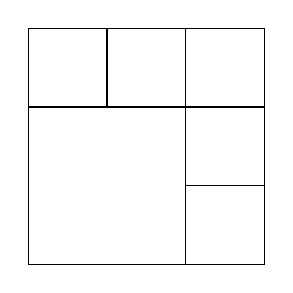
\begin{tikzpicture}

                \draw (0,0) -- (3,0) -- (3,3) -- (0,3) -- (0,0);
                \draw (2,0) -- (2,2) -- (0,2);
                \draw (1,2) -- (1,3);
                \draw (2,2) -- (2,3);
                \draw (2,1) -- (3,1);
                \draw (3,2) -- (2,2);

            \end{tikzpicture}
        \end{center}

        \textit{Hint: First show that any square subdivided into $k$ squares can easily be subdivided into $k+3$ squares, then think how many base cases you need to show are true.}

        \begin{solution}
            Let us prove show that any square can be subdivided into $n$ squares, where $n > 5$ and $n \in \Nat$ by induction. \\

            \textbf{Base Case} (n = 6) and (n = 7) \\

            Case: n = 6  \\
            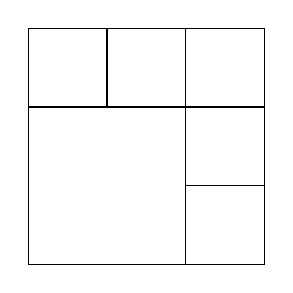
\begin{tikzpicture}
                \draw (0,0) -- (3,0) -- (3,3) -- (0,3) -- (0,0);
                \draw (2,0) -- (2,2) -- (0,2);
                \draw (1,2) -- (1,3);
                \draw (2,2) -- (2,3);
                \draw (2,1) -- (3,1);
                \draw (3,2) -- (2,2);
            \end{tikzpicture} \\

            Case: n = 7 \\
            \begin{tikzpicture}
                \draw (0,0) -- (4, 0) -- (4, 4) -- (0, 4) -- (0,0);
                \draw (0,2) -- (4,2);
                \draw (2,0) -- (2,4);
                \draw (1,0) -- (1,2);
                \draw (0,1) -- (2,1);
            \end{tikzpicture} \\

            Case: n = 8 \\
            \begin{tikzpicture}
                \draw (0,0) -- (4,0) -- (4,4) -- (0,4) -- (0,0);
                \draw (1,0) -- (1,4);
                \draw (0,1) -- (4,1);
                \draw (2,1) -- (2,0);
                \draw (3,1) -- (3,0);
                \draw (0,2) -- (1,2);
                \draw (0,3) -- (1,3);
            \end{tikzpicture}

            \textbf{Inductive hypothesis} \\
            Assume that a square can be represented with $k$ subdivisions \\

            \textbf{Inductive Step} \\
            Case 1: (k is even) \\
            If k is an even integer, the square can be represented in a form similar to that of (base case) n = 6, however instead of having one side consisting of 3 squares, it consists of k/2 squares (See Figure 1).

            In order to represent k + 1, decrement the number of boxes on two of its edges (ie given a square in the form of base case n = 6, update the square to be in a similar form however instead of each of the two sides having k/2 squares, update them to have k/2 - 1 squares or k-2 divisions for in total (See Figure 1). Then proceed to divide any of the squares into into 4 (See figure 2).

            \begin{figure}[H]
                \centering
                \includegraphics[width=0.5\linewidth, angle=90]{IMG_4025.JPG}
                \caption{form equivalent to base case n=6, however containing an side length of k/2 squares and k divisions total. }
                \label{fig:enter-label}
            \end{figure}


            \begin{figure}[H]
                \centering
                \begin{tikzpicture}
                    \draw (0,0) -- (4,0) -- (4,4) -- (0,4) -- (0,0);
                    \draw (6,0) -- (10,0) -- (10,4) -- (6,4) -- (6,0);
                    \draw (8,0) -- (8,4);
                    \draw (6,2) -- (10,2);
                \end{tikzpicture}
                \caption{Dividing a division/square into 4 subdivision aka creating 3 new division (k+3)}
            \end{figure}

            \begin{figure}[H]
                \centering
                \begin{tikzpicture}
                    \draw (0,0) -- (4,0) -- (4,4) -- (0,4) -- (0,0);
                    \draw (1,0) -- (1,4);
                    \draw (0,1) -- (4,1);
                    \draw (2,1) -- (2,0);
                    \draw (3,1) -- (3,0);
                    \draw (0,2) -- (1,2);
                    \draw (0,3) -- (1,3);
                \end{tikzpicture}
                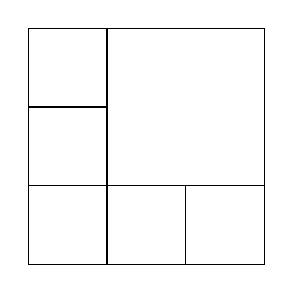
\begin{tikzpicture}
                    \draw (0,0) -- (3,0) -- (3,3) -- (0,3) -- (0,0);
                    \draw (1,0) -- (1,3);
                    \draw (0,1) -- (3,1);
                    \draw (2,1) -- (2,0);
                    \draw (0,2) -- (1,2);
                \end{tikzpicture}
                \caption{Creating/removing 2 subdivisions (k+2)}
            \end{figure}

            Case 2: (k is odd) \\
            If k is an odd integer, the square can be represented in the form shown in figure 4 (a composition of the outlined in figure 1 and figure 2.
            In order to subdivide a square into k+1 subdivisions, given a representation of k in the form described above, we can remove the divisions highlighted in red (in figure 4) (giving us a representation of k-3), then increment the divisions of each on each side by 2 (so what was previously $(k-3)/2$ becomes $(k-3)/2 + 2)$), increasing the total number of subdivisions by 4 in the process (giving us k+1 subdivision). \\


            \begin{figure}[H]
                \centering
                \includegraphics[width=0.5\linewidth]{IMG_4026.JPG}
                \caption{Representation of an odd number of subdivision}
                \label{fig:enter-label}
            \end{figure}

            \textbf{Conclusion} \\
            Given the assumption that a square can be divided into k square subdivisions, we have shown that through two cases (an odd and an even k) which can be represented as either in the form shown in figure 1 or the form shown in figure 4 (a combination of the forms in figure 1 and 2). If a square's k subdivisions is odd, it can be represented in a form similar to 4, meaning it contains a division shown in figure 2 (highlighted in red in figure 4), which can be removed. After removing this division (giving us k-3) we can create 2 subdivisions twice (operation represented in figure 3), in order it give us a total of k+1 subdivisions. However if the square contained an even k subdivisions, we can represent in in form represented in figure 1 (containing the edges lined with squares). In order to attain k+1 subdivisions we must decrement the number of squares lining two of the edges (the reverse of the operation outlined in figure 3), then subdivide any of the squares into 4 subdivisions (operation shown in future 2) (increasing the subdivision count by 3) giving us a total of k+1 subdivisions. $\qedsymbol$

            Note. The reasoning applies for k after the base case k = 8, because k=8 can be represented in a form with sufficient square subdivisions lining two of its edges such that the number can be decremented (operation in figure 3).  Use base cases for $k < 8$. \\
        \end{solution}
    \end{problem}
    \newpage

    \begin{problem}
        The Tribonacci numbers are defined by $T_0 = 1, T_1 = 1, T_2 = 2$, and $T_n = T_{n_1} + T_{n-2} + T_{n-3}$ for all $n \ge 3$. The beginning of the Tribonacci sequence is $1, 1, 2, 4, 7, 13, ...$.

        \subproblem Use strong induction to prove that $T_n \le 3^n$ for all natural numbers $n$.

        \subproblem Use strong induction to prove that any positive integer can be written as the sum of one or more \textit{distinct} Tribonacci numbers. For example, $3 = T_0 + T_2$, and $9 = T_0 + T_1 + T_4$. (Hint: consider the greatest $T_k$ less than $n+1$. Can you add other Tribonacci numbers to $T_k$ to reach $n+1$?)

        \begin{solution}
        (A) \\
        Let us prove with strong induction that $T_n \le 3^n$ for all natural numbers $n$.

        \textbf{Base Case} \\
        For n = 0, $T_0 = 1 \leq 3^0 = 1$: Case holds\\
        For n = 1, $T_1 = 1 \leq 3^1 = 3$: Case holds \\
        For n = 2, $T_2 = 1 \leq 3^2 = 9$: Case holds \\

        \textbf{Induction Hypothesis} \\
        According to strong induction we assume $T_k \leq 3^k$ for all natural number k less than or equal to n \\
        Therefore we can assume $T_n \leq 3^n, \quad T_{n-1} \leq 3^{n-1}, \quad T_{n-2} \leq 3^{n-2}$ \\

        \textbf{Induction step} \\
        Since $T_n \leq 3^n, \quad T_{n-1} \leq 3^{n-1}, \quad T_{n-2} \leq 3^{n-2}$ and $T_n = T_{n_1} + T_{n-2} + T_{n-3}$ we can sum the inequalities to achieve
        $T_{n+1} \leq 3^n + 3^{n-1} + 3^{n-2}$ \\
        $T_{n+1} \leq 3^{n-2} (3^2 + 3^1 + 3^0)$: factor out $3^{n-2}$ \\
        $T_{n+1} \leq 3^{n-2} * 13$ \\

        Now, $3^n \leq 3^{n-2} * 13$ because multiplying $3^{n-2}$ by 13 is less than multiplying $3^{n-2}$ by 9. Therefore, by  strong induction, $T_n \leq 3^n$ holds for all $n \geq 0$ \qedsymbol \\

        (B) \\
        Let us use strong induction to prove that any positive integer can be written as the sum of one or more \textit{distinct} Tribonacci numbers. \\

        \textbf{Base case} \\
        (n = 1): \\
        $1 = T_1$ \\

        (n = 2): \\
        $2 = T_2$ \\

        (n = 3): \\
        $3 = T_3$ \\

        \textbf{Induction hypothesis} \\
        Assume for all k where $1 \leq k \leq n$, each k an can be expressed as a sum of distinct Tribonacci numbers.

        \textbf{Induction Step} \\
        First we must find the largest Tribonacci number \( T_m \) such that \( T_m \leq n+1 \), then consider the number \( n+1 - T_m \).

        By the induction hypothesis, since \( n+1 - T_m \leq n \), \( n+1 - T_m \) can be expressed as a sum of distinct Tribonacci numbers. Therefore, we can write: $n+1 = T_m + (n+1 - T_m) $

        Since \( n+1 - T_m \) is expressible as a sum of distinct Tribonacci numbers by the induction hypothesis, and \( T_m \) is distinct from these numbers, \( n+1 \) is can also be expressed as a sum of distinct Tribonacci numbers.

        \textbf{Conclusion}
        By strong mathematical induction, we have shown that any positive integer \( n \) can be written as the sum of one or more distinct Tribonacci numbers \qedsymbol


        \end{solution}
    \end{problem}


\end{document}
